\documentclass[12pt]{standalone}
\usepackage{amsmath, amssymb, braket, xcolor, tikz}
\usetikzlibrary{calc, positioning, decorations.pathmorphing, arrows.meta}
\newlength\beamsplitterwidth\setlength\beamsplitterwidth{1.5em}
\newlength\wellwidth\setlength\wellwidth{2em}
\newlength\wellheight\setlength\wellheight{1.2\wellwidth}
\begin{document}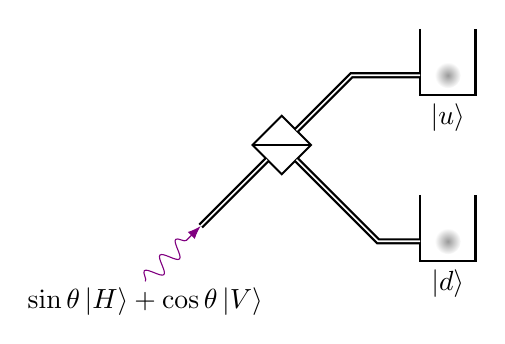
\begin{tikzpicture}[
    bs/.pic = {
        \coordinate (-c) at (0, 0);
        \path [draw=black, line width=0.7pt]
            (-.5\beamsplitterwidth, .5\beamsplitterwidth)
            -- ++(\beamsplitterwidth, 0) coordinate [midway] (-portt)
            -- ++(0, -\beamsplitterwidth) coordinate [midway] (-portr)
            -- ++(-\beamsplitterwidth, 0) coordinate [midway] (-portb)
            -- ++(0, \beamsplitterwidth) coordinate [midway] (-portl) -- cycle;
        \path [draw=black, line width=0.4pt]
            (-.5\beamsplitterwidth, .5\beamsplitterwidth)
            -- ++(\beamsplitterwidth, -\beamsplitterwidth);
    },
    well/.pic = {
        \path [draw=black, thick]
            (-.5\wellwidth, .5\wellheight)
            -- ++(0, -\wellheight)
            -- ++(\wellwidth, 0)
            -- ++(0, \wellheight);
        \node [circle, shading=radial, outer color=white, inner color=black!40!white, minimum width=.3\wellwidth] at (0, -.2\wellheight) {};
        \coordinate (-port) at (-.5\wellwidth, -.2\wellheight);
        \coordinate (-b) at (0, -.5\wellheight);
    },
    fibre/.style = {
        draw=black,
        thick,
        double,
    },
    photon/.style = {
        -Latex,
        draw=blue!50!red,
        decorate,
        decoration={
            snake,
            amplitude=.3em,
            segment length=.8em,
            post length=.5em,
        },
    },
]
\pic (bs) [rotate=45] {bs};
\pic (upper) at ($(bs-c) + (6em, 3em)$) {well};
\node [anchor=north, inner sep=0mm, yshift=-0.3em] at (upper-b) {$\ket u$};
\pic (lower) at ($(bs-c) + (6em, -3em)$) {well};
\node [anchor=north, inner sep=0mm, yshift=-0.3em] at (lower-b) {$\ket d$};
\path [fibre] ($(bs-portl) - (2.4em, 2.4em)$) coordinate (photon-in) -- (bs-portl);
\path let \p1=(bs-portr), \p2=(upper-port) in
    [fibre] (bs-portr) -- ++(\y2-\y1, \y2-\y1) -- (upper-port);
\path let \p1=(bs-portb), \p2=(lower-port) in
    [fibre] (bs-portb) -- ++(\y1-\y2, \y2-\y1) -- (lower-port);
\path [photon]
    ($(photon-in) - (2em, 2em)$)
    node [inner sep=0mm, anchor=north, yshift=-.21em] {$\sin\theta\ket H + \cos\theta\ket V$}
    -- (photon-in);
\end{tikzpicture}\end{document}
